\subsection{Absteigende motorische Bahnen}
Die Skelettmuskulatur, die für die Ausübung der willentlichen Bewegung des Körpers zu-ständig ist, wird direkt durch die sogenannten unteren Motorneurone innerviert. Ihre Zellkerne liegen innerhalb des Vorderhorns der grauen Substanz im Rückenmark. Die Aktivität dieser Motorneurone wird wiederum von den oberen Motorneuronen kontrolliert, welche dafür eine Reihe an absteigenden Bahnen hin zum Rückenmark und zu den Zellkernen der unteren Motorneurone bilden \textsuperscript{\cite[Kap.~1]{crossman2014neuroanatomy}}. Die absteigenden Bahnen können in zwei Hauptgruppen eingeteilt werden: In die lateralen und in die ventromedialen Bahnen des Rückenmarks. Die \textbf{lateralen Bahnen} bestehen aus dem \textit{Tractus corticospinalis} und dem \textit{Tractus rubrospinalis}. Sie sind an der Kontrolle der willkürlichen Motorik der distalen Muskulatur beteiligt. Die beiden Bahnen steigen an der lateralen Säule des Rückenmarks herab und terminieren in dorsolateralen Motorneuronenpools des Vorderhorns. Sie stehen unter cortikaler Kontrolle. Die \textbf{ventromedialen Bahnen} laufen in der ventromedialen Säule des Rückenmarks herab. Sie enden in ventromedialen Motorneuronenpools des Vorderhorns und sind hauptsächlich an der Kontrolle der Körperhaltung beteiligt. Hierzu zählt der \textit{Tractus reticulospinalis} und der \textit{Tractus vestibulospinalis}, welche durch den Hirnstamm innerviert werden (Abb.~\ref{fig:abst_Rueckenmark}) \textsuperscript{\cite[14]{neurowissenschaften_baer}}. 


\begin{figure}[H]
    \centering
    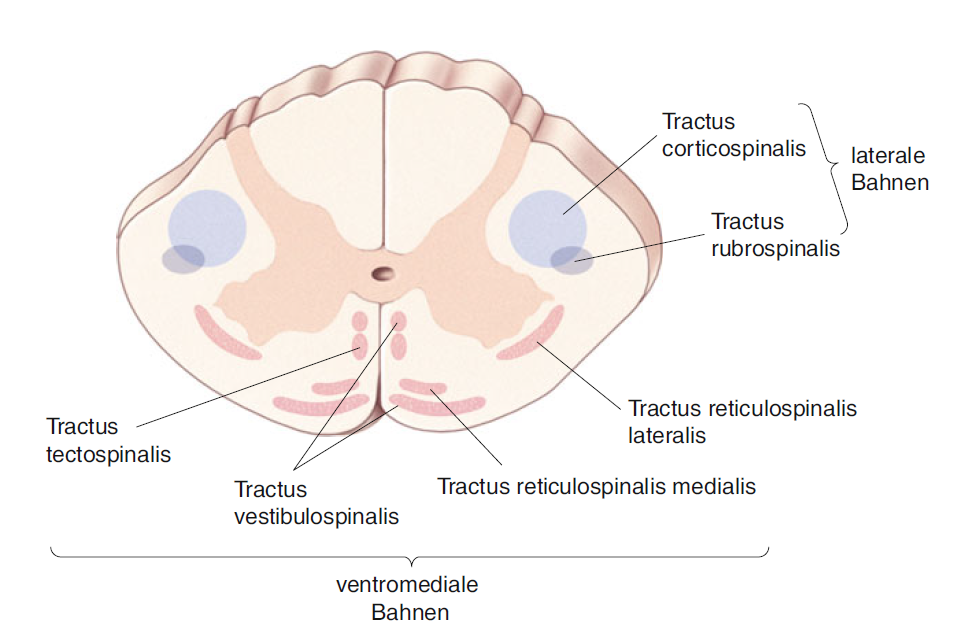
\includegraphics[width=1\textwidth]{pictures/Bilder_Laura/absteigende_bahnen_rkm.png}
    \caption[Absteigende Bahnen des Rückenmarks]{\textbf{Absteigende Bahnen des Rückenmarks.} Zu sehen ist die Lage der absteigenden motorischen Bahnen im Rückenmark. Die lateralen Bahnen, bestehend aus dem Tractus corticospinalis und dem Tractus rubrospinalis, liegen in der lateralen Säule des Rückenmarks. Die ventromedialen Bahnen bestehen aus dem Tractus reticulospinalis und Tractus vestibulospinalis und liegen ventromedial im Rückenmark. \\
    Abbildung aus \textit{Neurowissenschaften}, Bear et al. \textsuperscript{\cite[14]{neurowissenschaften_baer}}.}
    \label{fig:abst_Rueckenmark}
\end{figure}

\subsubsection{Tractus corticospinalis} \index{Tractus! corticospinalis} \label{subsubsec:corticospinalis}
Der \textbf{corticospinale Trakt} ist die größte absteigende Bahn mit etwa 10$^{6}$ Axonen und nimmt ihren Ursprung in der Großhirnrinde. Größtenteils entspringen die Axone dem \textbf{Motorkortex} der Großhirnrinde, aber ein Teil entstammt auch den somatosensorischen Arealen \textsuperscript{\cite[14]{neurowissenschaften_baer}}. 
Vom Großhirn ausgehend ziehen die Axone des corticospinalen Traktes in einem großen Faserbündel über die Capsula interna und stellen damit eine Verbindung zum Thalamus her. Dieser Fasertrakt verläuft dann weiter abwärts, über die Großhirnschenkel oder auch Crura cerebri des Mittelhirns und ventral entlang des Pons, bis zur Medulla oblongata \textsuperscript{\cite[8]{crossman2014neuroanatomy}}. Hier bildet der Fasertrakt eine markante Säulenstruktur an der ventralen Seite der Medulla, die auch von außen gut sichtbar ist. Diese Struktur wird oft als Pyramide bezeichnet, da sie im Querschnitt dreieckig erscheint. Sie gibt dem Tractus corticospinalis damit eine alternative Bezeichnung als Pyramidentrakt\index{Pyramidentrakt} (Abb.~\ref{fig:pyramidentrakt}) \textsuperscript{\cite[14]{neurowissenschaften_baer}}. An der caudalen Seite der Medulla kreuzen 75-90~\% der Fasern in der sogenannten \textbf{Pyramidenkreuzung} auf die contralaterale Seite in das Rückenmark und bilden damit den \textbf{Tractus corticospinalis lateralis}. Diese Bahn verläuft lateral in der weißen Substanz innerhalb des Rückenmarks abwärts und tritt dann Stück für Stück in den dorsolateralen Bereich des Vorderhorns der grauen Substanz ein. Hier befinden sich die zu innervierenden Motorneurone. Das Eintreten des lateralen corticospinalen Traktes in das Vorderhorn weist eine somatotopische Gliederung auf. Dies bedeutet, dass der medialst gelegene Bereich der Faserbahn zuerst in der Zervikalregion die Pyramidenbahn verlässt um in die graue Substanz einzutreten. Anschließend tritt dann der nun medial liegende Strang des corticospinalen Traktes in die thorakalen Vorderhörner ein. Dieses Vorgehen wird fortgeführt, bis der letzte Strang, der ursprünglich am lateralsten gelegen war, in die graue Substanz des Sakralmarks eintritt \textsuperscript{\cite[3]{trepel2011neuroanatomie}}. Der größte Teil, ca. 55~\%, der corticospinalen Neurone, ziehen in die zervikale Ebene und jeweils 20-25~\% der Neurone terminieren in der thorakalen oder lumbosakralen Ebene \textsuperscript{\cite[8]{crossman2014neuroanatomy}}. \\
\\ \noindent Auf Höhe der Pyramidenkreuzung bleiben 10-25~\% der pyramidalen Neurone ipsilateral und bilden damit den \textbf{Tractus corticospinalis anterior}. Dieser Faserstrang verläuft medial neben der Fissura longitudinalis in das  Rückenmark. Kurz bevor dieser Trakt im Zervikalmark endet, kreuzt er auf die contralaterale Seite und tritt dort in das Vorderhorn der grauen Substanz ein \textsuperscript{\cite[3]{trepel2011neuroanatomie}}. Damit bildet dieser Trakt sowohl im Ort der Kreuzung, als auch im Verlauf des Traktes im Rückenmark als Teil der lateralen Bahnen eine Ausnahme. \\
\\ \noindent Alle Fasern des corticospinalen Traktes enden im Vorderhorn in der grauen Substanz des Rückenmarks. Hier innervieren sie entweder über ein Interneuron oder auch direkt über eine synaptische Verbindung die $\upalpha$-Motorneurone, vor allem die der distalen Extremitätenmuskeln. Dem corticospinalen Trakt wird im Besonderen die Funktion der Kontrolle über freiwillige und feinmotorische Bewegungen zugesprochen \textsuperscript{\cite[3]{trepel2011neuroanatomie}}. \\
\\ \noindent In der Ratte jedoch ergeben sich einige Unterschiede bezüglich des Verlaufes und der Funktion des corticospinalen Traktes im Vergleich zu Primaten. Bis hin zur Pyramidenkreuzung in der Medulla oblongata ergeben sich keine Unterschiede. Nach der Kreuzung auf die contralaterale Seite in das Rückenmark allerdings, verläuft der Pyramidentrakt der Ratte in der dorsalen Säule der weißen Substanz nach unten und nicht lateral wie bei den Primaten. Des Weiteren endet dieser Strang nicht im Ventralhorn, sondern im medialen Bereich der grauen Substanz des Hinterhorns. Aufgrund dieser Terminationsstelle wird vermutet, dass der Pyramidentrakt in der Ratte keine markante Rolle in der Kontrolle der distalen Extremitäten wie bei Primaten einnimmt (Abb.~\ref{fig:tr_corticospinalis}) \textsuperscript{\cite[8]{paxinos2014rat}}.  

\begin{figure}[H]
    \centering
    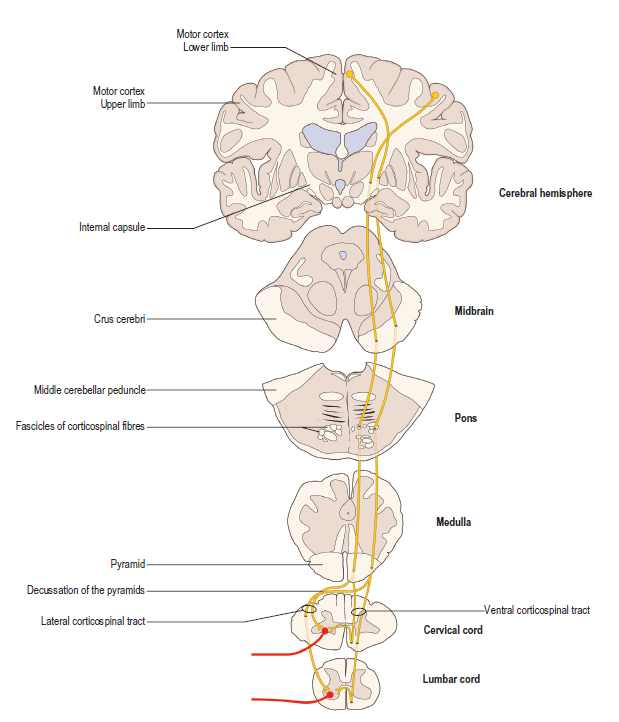
\includegraphics[width=0.85\textwidth]{pictures/Bilder_Laura/corticospinal_tract.PNG}
    \caption[Tractus corticospinalis]{\textbf{Tractus corticospinalis.} Der corticospinale Trakt entspringt dem Motorkortex der Großhirnrinde. Von dort verläuft er über die Capsula interna, die Crura cerebri (Mittelhirn) und ventral entlang des Pons zur Medulla oblongata. Hier teilt sich der Trakt in einen lateralen und anterioren Bereich. Der Tractus corticospinalis lateralis kreuzt in der Pyramidenkreuzung contralateral ins Rückenmark und zieht lateral in der weißen Substanz nach unten, bis er stufenweise in das Ventralhorn eintritt. Der Tractus corticospinalis anterior verläuft medial auf der ipsilateral Seite und kreuzt kurz bevor er im Vorderhorn des Zervikalmarks endet auf die contralaterale Seite. \\
    Abbildung aus \textit{Neuroanatomy}, Crossman und Neary \textsuperscript{\cite[8]{crossman2014neuroanatomy}}.}
    \label{fig:tr_corticospinalis}
\end{figure}

\begin{figure}[H]
    \centering
    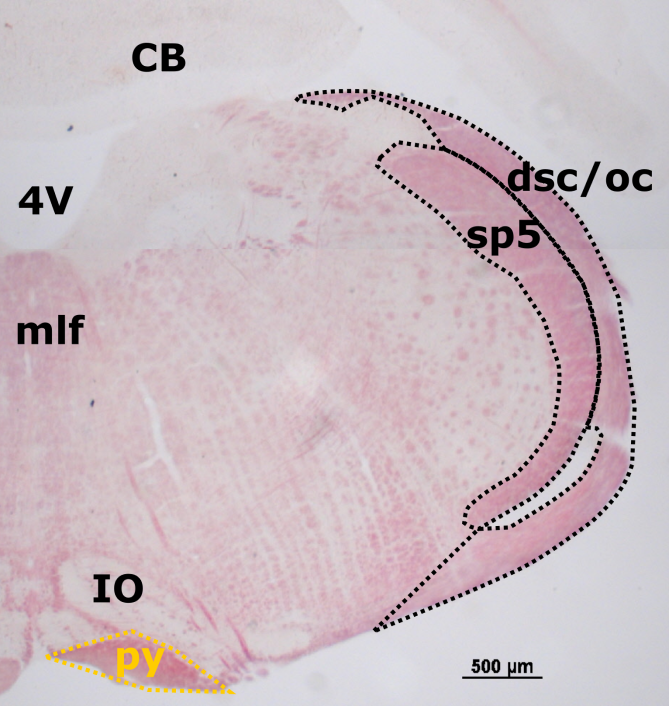
\includegraphics[width=0.5\textwidth]{pictures/Bilder_Laura/py_F04_2P_025x.png}
    \caption[Pyramidentrakt]{\textbf{Pyramidentrakt.} Der Tractus corticospinalis oder auch Pyramidentrakt (py) verläuft entlang der ventralen Seite des Hirnstamms, hier erkennbar durch das Cerebllum (CB) und den vierten Ventrikel (4V). Unterhalb des vierten Ventrikels zieht sich der Fasciculus longitudinalis medialis (mlf) durch den Hirnstamm. Oberhalb der Pyramidenbahn ist der untere Olivenkern (IO) zu erkennen. Seitlich des Hirnstamms ist der spinale Trakt des Trigeminusnerv (sp5), der dorsale Tractus spinocerebellaris (dsc) und der Tractus olivocerebellaris (oc) zu sehen. Faser-Färbung (F04-2).}
    \label{fig:pyramidentrakt}
\end{figure}

\subsubsection*{Der Motorcortex} \index{Cortex! Motorcortex}
Der Motorcortex befindet sich in der Großhirnrinde, genauer gesagt, liegt er im Frontallappen. Anterior zu dem Sulcus centralis \index{Sulcus! centralis}, der den Frontallappen vom Parietallappen abgrenzt, befindet sich der \textbf{Gyrus praecentralis} \index{Gyrus! praecentralis}. Dieser entspricht dem Brodmann Areal 4 oder auch funktionell gesehen dem \textbf{primären motorischen Cortex} \index{Cortex! primär motorisch} (\textbf{M1}). Innerhalb dieses Bereiches wird dabei die contralaterale Körperhälfte auf eine somatotopische Art und Weise repräsentiert. Dabei ist die Darstellung des Körpers umgedreht. Dies bedeutet, dass der Kopf im untersten Bereich des Gyrus praecentralis und die unteren Extremitäten an der medialen Oberfläche der Hemisphäre, direkt über dem Corpus callosum, repräsentiert sind. Körperteile, die dabei besonders fein differenziert sind, wie etwa die Hände, das Gesicht oder die Zunge, nehmen dabei deutlich größere Bereiche des Kortex ein (Abb.~\ref{fig:motorkortex}) \textsuperscript{\cite[13]{crossman2014neuroanatomy}}. Afferenzen erhält der Gyrus praecentralis hauptsächlich aus dem Nucleus ventralis anterolateralis, einer ventralen Kerngruppe des Thalamus. Dieses Kerngebiet leitet bereits vorverarbeitete motorische Impulse aus dem Cerebellum und den Basalganglia weiter. Efferenzen, die den primären motorischen Cortex verlassen, gehören hauptsächlich zum Tractus corticospinalis. Damit kontrolliert der Gyrus praecentralis über diesen Faserstrang die Willkürmotorik. Eine weitere Efferenz, die diesen Bereich verlässt, ist der Tractus corticonuclearis, welcher zu den Hirnnerven läuft und damit die Gesichtsmuskulatur steuert \textsuperscript{\cite[9]{trepel2011neuroanatomie}}. \\
Der Bereich anterior zum primären motorischen Cortex wird auch als \textbf{prämotorischer Cortex} \index{Cortex! prämotorisch} bezeichnet und entspricht dem Brodmann Areal 6. Die Region, die sich dabei auf der medialen Oberfläche der Hemisphäre in diesem Bereich befindet, wird als \textbf{supplementärmotorischer Cortex} \index{Cortex! supplementärmotorisch} abgegrenzt. Beide Bereiche ähneln in ihrer Verschaltung dem primären motorischen Cortex. Ihre Aufgabe besteht aber höchstwahrscheinlich mehr darin, Bewegungen zu programmieren und zu planen und die Körperhaltung zu kontrollieren (Abb.~\ref{fig:motorkortex}) \textsuperscript{\cite[13]{crossman2014neuroanatomy}}. 

\begin{figure}[H]
    \centering
    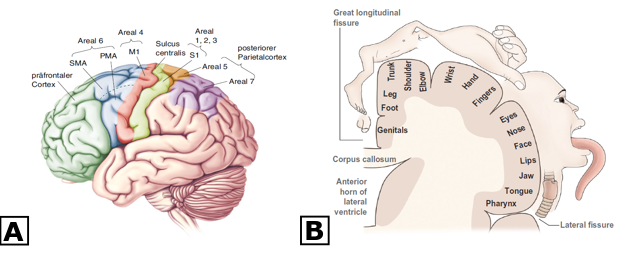
\includegraphics[width=\textwidth]{pictures/Bilder_Laura/Motorcortex_2.png}
    \caption[Motorcortex]{\textbf{Motorcortex.} \textbf{A:} Der motorische Cortex setzt sich aus dem primären motorischen Cortex (rot), dem prämotorischen Cortex und dem supplementärmotorischen Cortex (blau) zusammen. Der Gyrus praecentralis entspricht funktionell dem primären motorische Cortex. Anterior dazu befinden sich der prämotorische und supplementärmotorische Cortex. \\
    Abbildung aus \textit{Neurowissenschaften}, Bear et al. \textsuperscript{\cite[14]{neurowissenschaften_baer}}.\\ \textbf{B:} Der primäre motorische Cortex ist somatotopisch gegliedert. Der Kopfbereich ist dabei auf der unteren Hälfte und die Beine im oberen Bereich des Cortex abgebildet. Fein differenzierte Körperregionen nehmen dabei einen größeren Anteil der Oberfläche ein. \\
    Abbildung aus \textit{Neuroanatomy}, Crossman und Neary \textsuperscript{\cite[8]{crossman2014neuroanatomy}}.}
    \label{fig:motorkortex}
\end{figure}

\subsubsection*{Der Motorcortex der Ratte}
Wie bereits oben erklärt ist das Großhirn der Ratte lissencephal (Kap.~\ref{subsubsec:Grosshirnrinde}) und kann daher nicht anhand Gyri unterteilt werden.  
Allerdings kann der frontale Cortex der Ratte in drei Felder unterteilt werden: Fr1, Fr2 und Fr3. Dabei entspricht der Bereich des Fr1 funktionell dem primären motorischen Cortex mit Fr3 als somatotopisches Teilfeld. Fr2 ist das Äquivalent des prämotorischen und supplementärmotorischen Cortex (Abb.~\ref{fig:motorcortex_ratte}) \textsuperscript{\cite[22]{paxinos2014rat}}.  

\begin{figure}[H]
    \centering
    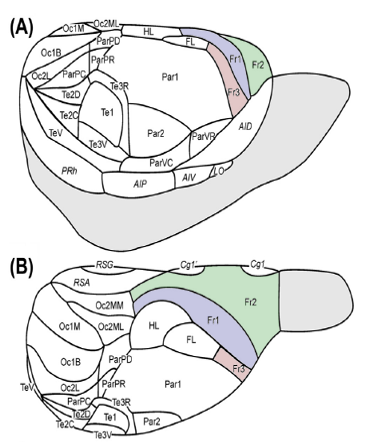
\includegraphics[width=0.5\textwidth]{pictures/Bilder_Laura/rat_motorcortex_1.png}
    \caption[Motorcortex Ratte]{\textbf{Motorcortex Ratte.} Schematische Zeichnung der \textbf{A} lateralen und \textbf{B} dorsalen Oberfläche eines Rattenhirns. Fr1 (blau) entspricht dem primären motorischen Cortex. Fr3 (rot) ist ein somatotopisches Teilfeld davon. Fr2 (grün) ist das Äquivalent zu den prämotorischen und supplementärmotorischen Arealen. \\ Abbildung aus \textit{The Rat Nervous System}, Paxinos et al. \textsuperscript{\cite[22]{paxinos2014rat}}.}
    \label{fig:motorcortex_ratte}
\end{figure}


\subsubsection*{Capsula interna} \index{Capsula interna}
Die \textbf{Capsula interna} ist eine große Ansammlung afferenter und efferenter Fasersysteme im Großhirnmarklager, die den Cortex mit subcortikalen Bereichen verbindet. Dieser Fasertrakt kann in unterschiedliche Bereiche unterteilt werden. Die absteigenden Bahnen des Motorkortex verlaufen im sogenannten \textit{Crus posterior} (hinterer Schenkel) der Capsula interna. Dieser Bereich weißt eine somatotopische Gliederung auf. Der corticospinale Trakt steigt hier in einer somatotopischen Reihe ab. Von vorne nach hinten verlaufen erst die oberen Extremitäten, gefolgt vom Rumpf und den unteren Extremitäten durch den hinteren Schenkel. Hier verlaufen auch die corticofugalen Fasern zu anderen motorischen Zentren im Hirnstamm. (Abb.~\ref{fig:Capsula_interna}) \textsuperscript{\cite[9]{trepel2011neuroanatomie}}.

\begin{figure}[H]
    \centering
    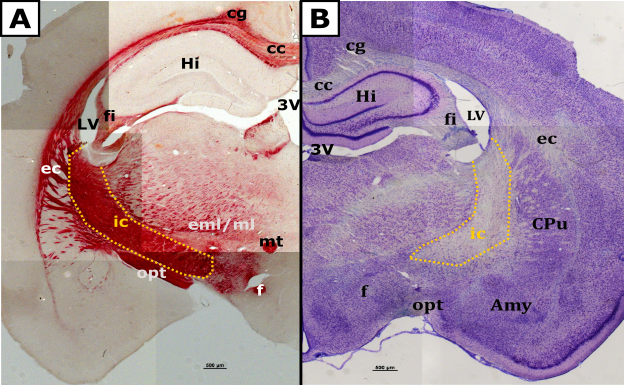
\includegraphics[width=\textwidth]{pictures/Bilder_Laura/internal_capsule_F21_3P_025x_N23_3P_025x.png}
    \caption[Capsula interna]{\textbf{Capsula interna.} \textbf{A:} Die Capsula interna (ic) liegt im Großhirnmarklager. Lateral in Richtung des Cortex ist die Capsula externa (ec) zu sehen. Des Weiteren sind auf dieser Abbildung erkennbar: Cingulum (cg), Corpus callosum (cc), Fimbria (fi), Fornix (f), Hippocampus (Hi), der laterale (LV) und dritte Ventrikel (3V), Tractus mammilothalamicus (mt), Lamina medullaris externa (eml), der mediale Lemniscus (ml) und der optische Trakt (opt). Faser-Färbung (F21-3). \textbf{B:} Die Capsula interna wird lateral durch das Caudateputamen (CPu) eingegrenzt. Darüber ist die Capsula externa (ec) zu erkennen. In dieser Abbildung sind außerdem zu sehen: Corpus callosum (cc), Cingulum (cg), Hippocampus (Hi), Fimbria (fi), Fornix (f), der laterale (LV) und dritte Ventrikel (3V), der optische Trakt (opt) und die Amygdala (Amy). Nissl-Färbung (N23-3).}
    \label{fig:Capsula_interna}
\end{figure}


\subsubsection*{Crura Cerebri} \index{Crura cerebri}
Die \textbf{Crura cerebri} oder auch Hirnschenkel besteht aus zwei Fasertrakten, welche vorne am Mittelhirn anliegen. In ihnen verlaufen Bahnen aus der Großhirnrinde, welche in den Hirnnervenkernen, im Rückenmark und in den Brückenkernen terminieren. Die Fibrae frontopontinae liegen dabei am medialsten. Ihnen schließen sich nach außen hin der Reihe nach der cortikonukleare Trakt, der cortocospinale Trakt und die Fibrae temporopontine, welche am lateralsten gelegen sind, an (Abb.~\ref{fig:crura_cerebri}) \textsuperscript{\cite[6]{trepel2011neuroanatomie}}.

\begin{figure}[H]
    \centering
    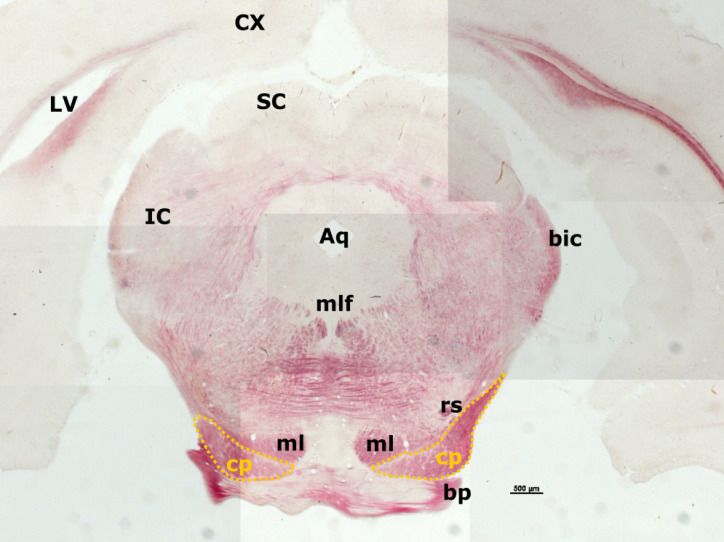
\includegraphics[width=0.7\textwidth]{pictures/Bilder_Laura/cerebral_peduncle_F14_4P_025x.png}
    \caption[Crura cerebri]{\textbf{Crura cerebri.} Die Crura cerebri sind ein Teil der Pedunculi cerebri (cp) und liegen dem Mittelhirn ventral-lateral an. Das Mittelhirn ist durch den Colliculus superior (SC), den Colliculus inferior (IC) und das Aquädukt (Aq) erkennbar. Oberhalb der Pedunculi cerebri sind der mediale Lemniscus (ml) und der Tractus rubrospinalis (rs) zu sehen. Weiterhin zu erkennen sind: der Fasciculus longitudinalis medialis (mlf), das Brachium pontis (bp), das Brachium des Colliculus inferior (bic), der Cortex (CX) und der laterale Ventrikel (LV). Faser-Färbung (F14-4).}
    \label{fig:crura_cerebri}
\end{figure}

\subsubsection{Tractus rubrospinalis} \index{Tractus! rubrospinalis} \label{subsubsec:rubrospinalis}
Der \textbf{Tractus rubrospinalis} geht aus dem \textbf{Nucleus ruber} (roter Kern) hervor, welcher im Tegmentum des Mittelhirns lokalisiert ist. Die Axone verlassen dieses Kerngebiet ventromedial und kreuzen in der \textit{Decussatio tegmentalis anterior} auf die contralaterale Seite. Anschließend verläuft der rubrospinale Trakt weiter bis er die Wirbelsäule erreicht, in der er in der lateralen Säule nach unten zieht. Er verläuft ventrolateral zum corticospinalen Trakt, bevor er in das Ventralhorn der grauen Substanz eintritt um Motorneurone zu innervieren. Der reticulospinale Trakt beeinflusst dabei die distalen Extremitätenmuskeln und ihren Tonus \textsuperscript{\cite[8]{crossman2014neuroanatomy}}. Im Menschen ist der rubrospinale Trakt schwach ausgebildet und reicht nur bis in das Zervikalmark. Die Kontrolle der distalen Muskulatur wird zum großen Teil durch den corticospinalen Trakt ausgeübt. In vielen anderen Säugerarten, unter anderem in der Ratte, spielt dabei aber der rubrospinale Trakt eine deutlich größere Rolle und ist auch dort stärker präsent. Es wird vermutet, dass dieser im Verlauf der Primatenevolution durch den Pyramidentrakt weitestgehend ersetzt wurde (Abb.~\ref{fig:tr_rubrospinalis}, Abb.~\ref{fig:rubrospinal_tract}) \textsuperscript{\cite[14]{neurowissenschaften_baer}}. 
\begin{figure}[H]
    \centering
    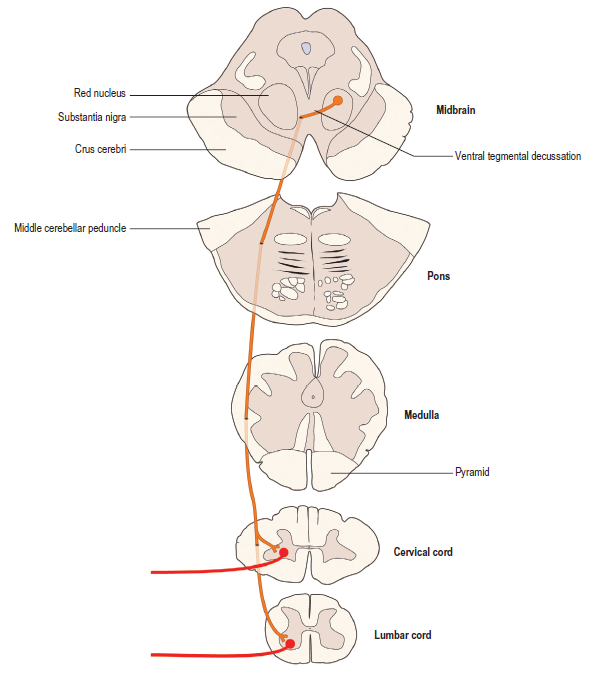
\includegraphics[width=0.85\textwidth]{pictures/Bilder_Laura/rubrospinal_tract.PNG}
    \caption[Tractus rubrospinalis]{\textbf{Tractus rubrospinalis.} Der Tractus rubrospinalis entspringt dem Nucleus ruber, welcher im Mittelhirn lokalisiert ist. Von dort kreuzt er in der Decussatio tegmentalis anterior auf die contralaterale Seite und steigt in der lateralen Säule das Rückenmark hinab, bis er in das Vorderhorn eintritt. \\
    Abbildung aus \textit{Neuroanatomy}, Crossman und Neary \textsuperscript{\cite[8]{crossman2014neuroanatomy}}.}
    \label{fig:tr_rubrospinalis}
\end{figure}

\begin{figure}[H]
    \centering
    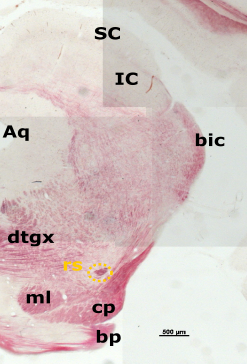
\includegraphics[width=0.5\textwidth]{pictures/Bilder_Laura/rubrospinal_tract_F14_4P_025x.png}
    \caption[Tractus rubrospinalis Querschnitt]{\textbf{Tractus rubrospinalis Querschnitt.} Der Tractus rubrospinalis (rs) entspringt dem Nucleus ruber des Mittelhirns und verläuft von dort ventro-medial. Das Mittelhirn ist durch den Colliculus superior (SC), den Colliculus inferior (IC) und das Aquädukt (Aq) erkennbar. In der Abbildung sind weiterhin zu sehen: die Pedunculi cerebri (cp), der mediale Lemniscus (ml), die dorsale Kreuzung des Tegmentums (dtgx), das Brachium pontis (bp) und das Brachium des Colliculus inferior (bic). Faser-Färbung (F14-4).}
    \label{fig:rubrospinal_tract}
\end{figure}


\subsubsection*{Nucleus ruber} \index{Nucleus! ruber}
Der \textbf{Nucleus ruber} oder auch \textbf{roter Kern} hat seinen Namen anhand seiner markanten roten Färbung erhalten. Dieser Farbton entsteht aufgrund eines sehr hohen Eisengehalts in den dort vorhandenen Zellkernen. Er ist in der Mitte des Tegmentum im Mittelhirn, auf selber Höhe wie der Superior colliculus, lokalisiert. Histologisch kann das Kerngebiet in einen kleinzelligen (\textit{Pars parvocllularis}) und einen großzelligen (\textit{Pars magnocellularis}) Bereich eingeteilt werden. Afferenzen empfängt der rote Kern zum einen durch Fasern des ipsilateralen Motorkortex des Frontallappens und zum anderen aus den Kerngebieten der contralateralen Kleinhirnhälfte. Damit ist der Nucleus ruber eine zentrale Schaltstelle des motorischen Systems, der zum einen für eine glatte Ausführung von Willkürbewegungen sorgt, aber auch die Körperhaltung und den Muskeltonus beeinflusst. Diese Information wird in Efferenzen über den Tractus rubrospinalis zu den Muskeln geleitet. Zusätzlich existieren Efferenzen, die über den Tractus tegmentalis centralis zum unteren Olivenkernkomplex projizieren. Von dort findet eine Weiterleitung der Information an das Cerebellum statt, um dann wieder zurück in den Nucleus ruber oder in den Thalamus zu gelangen. In dieser Feedback-Schleife findet eine Modifikation und Bearbeitung der motorischen Information statt, bevor sie in das Rückenmark geleitet wird (Abb.~\ref{fig:roter_Kern}) \textsuperscript{\cite[6]{trepel2011neuroanatomie}}. 

\begin{figure}[H]
    \centering
    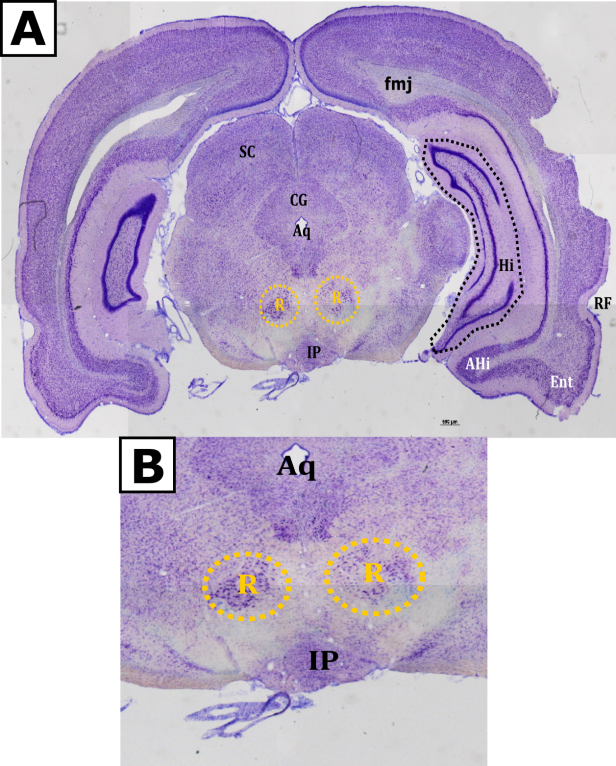
\includegraphics[width=0.6\textwidth]{pictures/Bilder_Laura/red_nucleus_N16_3P_025x.png}
    \caption[Nucleus ruber]{\textbf{Nucleus ruber.} \textbf{A:} Der Nucleus ruber (R) liegt ventral-medial im Mittelhirn auf selber Höhe wie der Colliculus superior (SC). Unterhalb des roten Kerns ist der Nucleus interpeduncularis (IP) zu erkennen. Das Aquädukt (Aq) wird vom zentralen Höhlengrau (CG) umgeben. Der Cortex, welcher sich hier aus dem  amygdalo-hippocampalen Bereich (AHi), dem Cortex entorhinalis (Ent), dem Forceps major des Corpus callosum (fmj) und dem Hippocampus (Hi) zusammensetzt, umgibt das Mittelhirn. \textbf{B:} Detailausschnitt des Nucleus ruber (R). Oberhalb ist das Aquädukt (Aq) und unterhalb der Nucleus interpeduncularis (IP) zu erkennen. Nissl-Färbung (N16-3).}
    \label{fig:roter_Kern}
\end{figure}

\subsubsection{Tractus reticulospinalis} \index{Tractus! reticulospinalis} \label{subsubsec:reticulospinalis}
Der \textbf{Tractus reticulospinalis} kann in zwei Bahnen unterteilt werden, den \textbf{Tractus reticulospinalis medialis} und den \textbf{Tractus reticulospinalis lateralis}. Beide haben ihren Ursprung in der medialen Zone der \textit{Formatio reticularis} des Hirnstamms. Die Axone des medialen Reticulospinaltrakts entstammen der pontinen Formatio reticularis und steigen ipsilateral im Vorderstrang der weißen Substanz im Rückenmark ab. Aus der medullären Formatio reticularis entsteht der laterale Tractus reticulospinalis. Dieser zieht bilateral im Vorderstrang des Rückenmarks nach unten \textsuperscript{\cite[8]{crossman2014neuroanatomy}}. Beide Bahnen haben die Funktion das Gleichgewicht zu halten, indem sie die Körperhaltung kontrollieren. Die beiden Bahnen wirken dabei entgegengesetzt. Der mediale Faserstrang beeinflusst die Muskulatur der Extensoren und der laterale Tractus reticulospinalis kontrolliert die Flexorenmuskulatur (Abb.~\ref{fig:tr_reticulospinalis}) \textsuperscript{\cite[14]{neurowissenschaften_baer}}.


\begin{figure}[H]
    \centering
    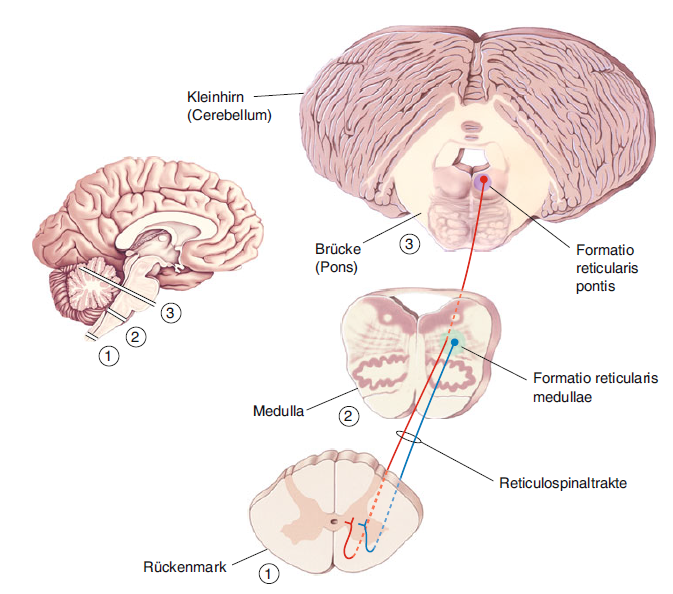
\includegraphics[width=0.68\textwidth]{pictures/Bilder_Laura/reticulospinaler_tract.PNG}
    \caption[Tractus reticulospinalis]{\textbf{Tractus reticulospinalis.} Den reticulospinalen Trakt kann man in zwei Faserstränge unterteilen. Der Tractus reticulospinalis medialis entstammt der pontinen Formatio reticularis und der Tractus reticulospinalis lateralis geht aus der medullären Formatio reticularis hervor. Beide Faserstränge ziehen im Vorderstrang des Rückenmarks nach unten. Abbildung aus \textit{Neurowissenschaften}, Bear et al. \textsuperscript{\cite[14]{neurowissenschaften_baer}}.}
    \label{fig:tr_reticulospinalis}
\end{figure}

\subsubsection*{Formatio reticularis} \index{Formatio reticularis}
Die \textbf{Formatio reticularis} ist ein komplexes Netz an Neuronen, welches sich über die gesamte Länge des Hirnstammtegmentums erstreckt. Damit ist dieser Bereich phylogenetisch betrachtet ein sehr alter Bereich des Hirnstamms, der unter anderem für die Koordination lebensnotwendiger Funktionen zuständig ist \textsuperscript{\cite[6]{trepel2011neuroanatomie}}. Die darin enthaltenen Kernbereich sind zum Teil diffus und schwer von einander abzugrenzen und manche Funktionen, wie beispielsweise das Atmungs- und das Kreislaufsystem, werden durch neuronale Netzwerke und nicht durch anatomisch abgegrenzte Bereiche gesteuert \textsuperscript{\cite[9]{crossman2014neuroanatomy}}. 
%Zwei Kernregionen lassen sich jedoch gut von den restlichen Strukturen abgrenzen, die Raphé-Kerne und der Locus coeruleus (Kap.~\ref{serotonerges_system}, Kap.~\ref{fig:noradrenerges_system}). In die Längsrichtung lässt sich die Formatio reticularis in drei Zonen unterteilen. Die erste ist die mediane Zone, welche aus den oben genannten Raphé-Kernen besteht. An diesen Bereich grenzen seitlich zum einen die mediale Zone, bestehend aus sehr großzelligen Kernen, und zum anderen die laterale Zone mit sehr kleinzelligen Kernen an \textsuperscript{\cite[6]{trepel2011neuroanatomie}}. 
Es gibt ein breites Spektrum an afferenten und efferenten Verbindungen der Formatio reticularis. Der Bereich in der Medulla und dem Pons erhält besonders viel Input aus dem prämotorischen Cortex, dem Cerebellum und dem limbischen System. Aus diesem Gebiet entsteht die absteigenden Bahnen des Tractus reticulospinalis. Der mediale reticulospinale Trakt bildet sich aus der pontinen Formatio reticularis und der laterale reticulospinale Trakt geht vom medullären Bereich aus. Dort befinden sich Zellgruppen mit besonders großen Zellkörpern, die \textit{Nucleus reticularis gigantocellularis} genannt werden. Aus ihnen gehen die Fasern des lateralen Traktes hervor. Über die reticulospinalen Bahnen nimmt die Formatio reticularis Einfluss auf den Muskeltonus und Bewegungen der proximalen Extremitäten und des Rumpfes \textsuperscript{\cite[9]{crossman2014neuroanatomy}}.
\newpage
\subsubsection{Tractus vestibulospinalis} \index{Tractus! vestibulospinalis} \label{subsubsec:vestibulospinalis}
Die Fasern des \textbf{Tractus vestibulospinalis} entspringen den \textit{Nuclei vestibulares}, die sich im Pons und der Medulla oblongata befinden. Dieses Kerngebiet erhält seine Informationen aus dem Gleichgewichtsorgan des Innenohrs über Afferenzen des Nervus vestibularis und auch aus dem Kleinhirn. Dem lateralen Vestibulariskern, auch Deiters Kern genannt, entspringen Fasern, welche als \textbf{lateraler vestibulospinaler Trakt} ipsilateral im Vorderstrang des Rückenmarkes über Zervikal- und Thorakalsegmene bis nach unten ins Lumbalmark ziehen. Über eine Erregung der Motorneurone der Beinextensorenmuskulatur wird die Muskelspanung kontrolliert um die Körperhaltung, sowie das Gleichgewicht aufrecht zu halten. Aus dem medialen Vestibulariskern entsteht der \textbf{mediale vestibulospinale Trakt}. Dieser Faserstrang zieht bilateral im Vorderstrang des Rückenmarks bis in die Zervikal- und Thorakalsegmente. Er aktiviert die Motorneurone, die die Hals- und Rückenmuskulatur innervieren, um die Kopfposition in Relation zum Körper zu koordinieren \textsuperscript{\cite[14]{neurowissenschaften_baer},\cite[9]{crossman2014neuroanatomy},\cite[8]{paxinos2014rat}}.  


\begin{figure}[H]
    \centering
    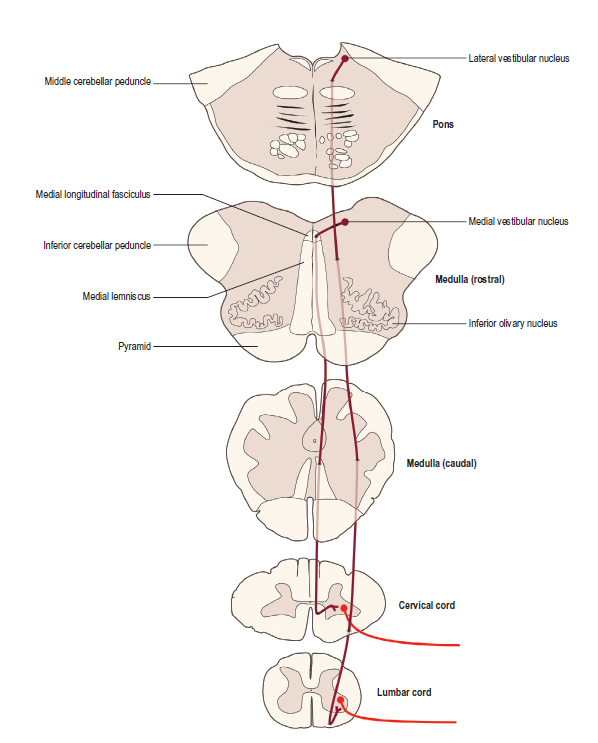
\includegraphics[width=0.65\textwidth]{pictures/Bilder_Laura/vestibulospinal_tract.PNG}
    \caption[Tractus vestibulospinalis]{\textbf{Tractus vestibulospinalis.} Die Fasern des Tractus vestibulospinalis entstammen den Vestibulariskernen, die im Hirnstamm lokalisiert sind. Aus dem lateralen Vestibulariskern in dem Pons entstammen die Axone, die als lateraler vestibulospinaler Trakt ipsilateral im Vorderstrang des Rückenmarks bis nach unten in das Lumbalmark ziehen. Der mediale vestibulospinale Trakt entsteht aus dem medialen Vestibulariskern in der Medulla. Dieser Faserstrang zieht bilateral zu den Zervikal- und Thorakalsegementen der Wirbelsäule. Abbildung aus \textit{Neuroanatomy}, Crossmann und Neary \textsuperscript{\cite[8]{crossman2014neuroanatomy}}.}
    \label{fig:tr_vestibulospinalis}
\end{figure}

% \subsubsection*{Nuclei vestibulares} \index{Nuclei! vestibulares}
% Die \textbf{Nuclei vestibularis} sind eine von zwei Kerngruppen die von dem XIII. Hirnnerv, dem Nervus vestibulocochlearis, ihren Input erhalten. Die eingehenden Informationen bestehen aus Lage- und Beschleunigungsparametern der Vestibularorgane des Innenohrs. Die Vestibulariskerne bestehen aus vier Kernen, superior, inferior, medialis und lateralis, die sich in ihrer Funktion unterscheiden. Zusätzlich erhalten diese Kerngruppen auch Informationen aus dem Kleinhirn und sogar aus dem Rückenmark. Von den Vestibulariskernen ausgehend gibt es Efferenzen, die diesen Input dann an den Thalamus, in das Cerebellum, zu Augenmuskelkernen, zu Zentren der Formatio reticularis und über den Tractus vestibulospinalis auch zum Rückenmark leiten. Die wichtigste Aufgabe dieser Kerngruppen ist die Verarbeitung der einkommenden Informationen des Vestibularogans, um damit Korrekturbewegungen einzuleiten und den Körper im Gleichgewicht zu halten. Eine weitere Funktion ist auch die Blickstabilisierung, wenn sich der Körper bewegt \textsuperscript{\cite[5]{trepel2011neuroanatomie}}.  
